\documentclass[notitlepage, 12pt]{article}
\usepackage[english]{babel}           % LANGEUAGE=ENGLISH, UTF-8
\usepackage[utf8]{inputenc}
\usepackage[T1]{fontenc}
\usepackage{amsmath}                  % ALL MATH FEATURES
\usepackage{graphicx}                 % GRAPHICS                  
\usepackage{float}                    % IMPROVED FIGURE POSITIONING
\usepackage[labelsep=period,labelfont=bf]{caption} % IMPROVED CAPTIONS
\usepackage{url}                      % WRITE URLS
\usepackage{tikz}                     % MAKE TIKZ VECTOR GRAPHICS
\usepackage{tocloft}                  % CONTROL TABLE OF CONTENTS
\usepackage[authoryear,round]{natbib} % REFERENCES
\usepackage{apalike}
\usepackage{pdflscape}                % USE LANDSCAPE MODE
\usetikzlibrary{decorations.pathreplacing}
\usepackage{enumitem}


\usepackage{algorithm}
\usepackage{algorithmicx}
\usepackage{algpseudocode}


\renewcommand{\familydefault}{lmr}           % SET DOCUMENT FONT
\makeatletter                         
\renewcommand{\section}{\@startsection       % SECTION
        {section}
        {2}
        {0mm}
        {1.2\baselineskip}
        {\baselineskip}
        {\centering\normalsize}}
\renewcommand{\subsection}{\@startsection    % SUBSECTION
        {subsection}
        {2}
        {0mm}
        {.8\baselineskip}
        {.5\baselineskip}
        {\bfseries\normalsize}}
\renewcommand{\subsubsection}{\@startsection % SUBSUBSECTION
        {subsubsection}
        {2}
        {0mm}
        {.5\baselineskip}
        {0mm}
        {\it\bfseries\normalsize}}
\makeatother
    
% define algorithm environments
\floatstyle{plaintop}
\newfloat{algorithm}{bpht}{alg}
\floatname{algorithm}{Algorithm}

%define title matter
\title{Simulating a dark matter halo using a parallel grid method}
\author{{\em Otto Hannuksela} \and {\em Janne Lampilahti}}
\date{\today}

\begin{document}
\maketitle
\section{INTRODUCTION}
Dark matter appears to be the dominant form of matter in the universe. While no direct observations of dark matter exist, it has been observed indirectly through its gravitational interaction with visible matter and radiation \citep{Roos2010}. The effect of dark matter on structure formation in the universe is the subject of an increasing scientific interest and a useful tool in the search for possible candidates of dark matter. Current progress in the investigation of structure formation is mainly driven by advances in computational methods and capabilities \citep{Kuhlen2012}. 

In this work we simulate a dark matter halo, neglecting baryonic matter, by using a particle based method and solving the Poisson's equation of gravity. The software used is {\em Uintah} (available from \url{http://uintah.utah.edu/} during the writing of this report), a parallel grid framework with a support for particle interactions and adaptive mesh refinement and which is aimed at solving partial differential equations. A major part of the project was to learn how to use the tools provided by Uintah.

\section{METHODS} \label{sec:methods}

In this section the relevant theory and numerical methods are described. The method in short was to use a Poisson solver operating on a grid and an $N$-body integrator operating on particles, that are coupled via interpolation between the grid and the particles. This method is used in the context of massive collisionless particles interacting through gravity \citep[e.g.][]{Hockney1985}.  

%%%%%
\subsection{Theory}
A distribution of mass density $\rho$ gives rise to a gravitational potential $\phi$ according to the Poisson's equation of gravity
\begin{equation}
\nabla^2 \phi = 4\pi G \rho,
\end{equation}
where $G\approx 6.674\times10^{-11}$ Nm$^2$/kg$^2$ is the gravitational constant. In our simulation we normalize $G=1$. The corresponding force field can be solved from the gradient
\begin{equation}
\mathbf{F} = -\nabla \phi.
\end{equation}
In our simulation a distribution of massive particles create the mass density. A new position and velocity for the particles after a time step $dt$ can be solved from the Newton's equation of motion.
\begin{align}
\mathbf{v}(t+dt) &= \int_{t}^{t+dt}\frac{\mathbf{F}(t')}{m}dt' +  \mathbf{v}(t)\\
\mathbf{x}(t+dt) &= \int_{t}^{t+dt}\mathbf{v}(t')dt' +  \mathbf{x}(t)
\end{align}
The use of this theory assumes that we do not have relativistic speeds or masses and that the maximum grid size is small enough that expansion of the universe can be neglected.

One approach would be to try to calculate the particle-particle interactions but this is not computationally feasible since we would have $2^N$ interactions where $N$ is the particle number and we are using thousands of particles.  

%%%%%
\subsection{Numerical methods}\label{ssec:numerical}
The simulation is set up with respect to a three dimensional grid that supports particles (Fig. \ref{fig:grid}).
The overall algortihm is expressed in Algortihm \ref{alg:main}.
\begin{algorithm}[H]
\hspace{0.1\textwidth}\parbox{.8\textwidth}{
\-\hspace{0ex}set Dirichlet or periodic boundary conditions\\
\-\hspace{0ex}set initial $\mathbf{x}_p$, $\mathbf{v}_p$ and $m_p$ for all particles $p$\\
\-\hspace{0ex}interpolate initial $\rho$ from particle mass $m_p$\\
\-\hspace{0ex}set initial guess for $\phi$\\
\-\hspace{0ex}{\bf loop}\\
\-\hspace{4ex}solve $\phi$ at the nodes using the Jacobi method\\
\-\hspace{4ex}calculate $\mathbf{F}=-\nabla \phi$ with respect to each particle $p$\\
\-\hspace{4ex}{\bf for} every particle $p$ {\bf do}\\
\-\hspace{8ex}$\mathbf{v}_p(t+\Delta t) = (\mathbf{F}_p/m)\Delta t + \mathbf{v}_p(t)$\\
\-\hspace{8ex}$\mathbf{x}_p(t+\Delta t) = \mathbf{v}_p(t)\Delta t + \mathbf{x}_p(t)$\\
\-\hspace{4ex}{\bf end for}\\
\-\hspace{4ex}interpolate new $\rho$ from particle mass $m_p$\\
\-\hspace{4ex}$t\leftarrow t+\Delta t$\\
\-\hspace{0ex}{\bf end loop}}
\caption{Main program.}
\label{alg:main}
\end{algorithm}

The Poisson's equation of gravity is discretized to 
\begin{equation} \label{eq:discretized_poisson}
\begin{aligned}
4\pi G\rho_{i,j,k} &= \frac{\phi_{i+1,j,k}-2\phi_{i,j,k}+\phi_{i-1,j,k}}{(\Delta x)^2}+\\
& \phantom{{}={}} \frac{\phi_{i,j+1,k}-2\phi_{i,j,k}+\phi_{i,j-1,k}}{(\Delta y)^2}+\\
& \phantom{{}={}} \frac{\phi_{i,j,k+1}-2\phi_{i,j,k}+\phi_{i,j,k-1}}{(\Delta z)^2}.
\end{aligned}
\end{equation}


The gravitational potential $\phi$ is then solved at each node using using the Jacobi method (Algorithm \ref{alg:Jacobi}) . In the calculation of the potential gradient we obtain the potential values near the particles by linear interpolation and then calculate the gradient by numerical differentiation. For exmaple at the $p$th particle the gradient is calculated in the $x$ direction as

\begin{equation}
(\nabla \phi)(x_p)=\frac{\phi(x_p+dx)-\phi(x_p-dx)}{2dx},
\end{equation}
where $x_p$ is the particle's $x$ coordinate and $dx$ is a small distance.  

The particle velocity and position are evolved over a small time step $dt$, assuming that the force remains constant. Essentially this means calculating for each particle
\begin{align}
&=\mathbf{v}_p(t+\Delta t) = (\mathbf{F}_p/m)\Delta t + \mathbf{v}_p(t)\\
&=\mathbf{x}_p(t+\Delta t) = \mathbf{v}_p(t)\Delta t + \mathbf{x}_p(t).
\end{align}
After this using the new positions the particle masses are linearly interpolated back to the nodes to obtain a new mass density $\rho$.

\begin{algorithm}[H]
\hspace{0.1\textwidth}\parbox{.8\textwidth}{
\-\hspace{0ex}{\bf function} Jacobi($\phi$, tolerance, max\_iterations)\\
\-\hspace{4ex}{\bf for} $n = 0,1,\ldots\mbox{max\_iterations}$ {\bf do}\\
\-\hspace{8ex}error $\sigma\leftarrow 0$\\
\-\hspace{8ex}{\bf for} every node $\phi_{i,j,k}$\\
\-\hspace{12ex}$\phi_{i,j,k}^{(n+1)} \leftarrow \phi_{i,j,k}^{(n)} + (\phi_{i+1,j,k}^{(n)} +\phi_{i-1,j,k}^{(n)}+$\\
\-\hspace{12ex}$\phantom{\phi_{i,j,k}^{(n+1)} \leftarrow }\phi_{i,j+1,k}^{(n)}+ \phi_{i,j-1,k}^{(n)} + \phi_{i,j,k+1}^{(n)} + \phi_{i,j,k-1}^{(n)} +$\\
\-\hspace{12ex}$\phantom{\phi_{i,j,k}^{(n+1)} \leftarrow} h^2\rho_{i,j,k})$\\
\-\hspace{12ex}update $\sigma$\\
\-\hspace{8ex}{\bf end for}\\
\-\hspace{8ex}{\bf if} $\sigma \leq $ tolerance, {\bf break}\\
\-\hspace{4ex}{\bf end for}\\
\-\hspace{4ex}{\bf return} $\phi$\\
\-\hspace{0ex}{\bf end function}}
\caption{Calculating potential $\phi$ using the Jacobi algorithm.}
\label{alg:Jacobi}
\end{algorithm}




%%%%%
\subsection{Initialization of the simultaion}
The specific case we want to study with our simulation is a dark matter halo. Dark matter halos are structures composed of dark matter, believed to envelope galaxy disks.

We randomly distribute dark matter particles into a box and let them collapse by the effect of gravity. We used either Dirichlet boundary conditions with $\rho=0$ or periodic boundary conditions.    

%%%%%
\subsection{Verification of results} \label{sec:verification}
To verify the simulation results we test for energy conservation:
\begin{equation}
\begin{aligned}
T+V&=\mathrm{constant}\\
\frac{1}{2}\sum_{p} m_pv_p^2 + M\sum_{i,j,k}\phi_{i,j,k} &= \mathrm{constant} 
\end{aligned}
\end{equation}
where $T$ is the total kinetic energy, $V$ is the total potential energy and $M$ refers to the total mass of the particles. In the context of gravitationl interactions only, the virial theorem states:
\begin{equation}
\langle T \rangle_\tau = -\frac{1}{2}\langle V \rangle_\tau
\end{equation}
where we take a time average of the kinetic and potential energy over a time period $\tau$.


We could not use time steps, distances or masses with proper units because the Uintah interpolator had some problems with large numerical values (see section \ref{ssec:Uintah}). Therefore the set of values in our simulation have arbitrary units. To test energy conservation we solved a scaling factor $c$ from the virial theorem over some time interval $\tau$. The scaling factor relates the kinetic energy $T$ and potential energy $V$ of the system via $\langle T \rangle_{\tau}$=c$\langle V\rangle_{\tau}$. We then tested whether energy conservation is satisfied when we use the scaling factor $c$.  

We also compared the radial mass distribution of the obtained halo with the Navarro-Frenkel-White (NFW) profile, which is the radial mass distribution often obtained from simulations \citep{Navarro1995}. The profile is given by  
\begin{equation}
\rho(r) = \frac{\rho_0}{\frac{r}{R_s}\left(1 + \frac{r}{R_s}\right)^2},
\label{eq:nfw}
\end{equation}
where $r$ is distance from the center of the halo and $(\rho_0,R)$ are parameters.    

\section{IMPLEMENTATION}

In this section, we will often refer to Section \ref{ssec:numerical} and describe each numerical method's implementation in detail. During the whole 
project, we made a lot of effort to make sure the algorithms fit the Uintah framework. Because of this, we will have extensive description of 
the Uintah framework in the Section \ref{ssec:Uintah}, describing how the Uintah patches which are used in the Poisson solver work, 
how particle masses are interpolated to the grid and how the gradient of potential is calculated. 

In addition to describing our implementation and the Uintah framework, 
we will discuss some of the limitations and 
bugs of Uintah software which drained a painstaking amount of time to solve. For more information on Uintah framework, please refer to the \emph{uintah\_presentation.pdf} 
we made on the software.

\subsection{Uintah} \label{ssec:Uintah}
% describe uintah

As mentioned in the title, we made a \emph{fully parallel} poisson solver utilizing particle-in-cell approach.

Before we start with the actual algorithms, let's go through the basics of Uintah. There are a few concepts to understand; \emph{cells}, \emph{patches}, 
\emph{ghost cells}, \emph{cell-centered variables}, \emph{node-centered variables}, \emph{face-centered variables} and \emph{particles}. 

We present an explanation for each of these accompanied by a Figure (Figure \ref{fig:grid}) demonstrating a visual description.

\begin{enumerate}
\item \emph{Cells} are finite boxes in the grid. These are the basic elements of our simulation. In the case of our poisson solver, we discretize our poisson equation 
based on cells in such a way that our discretization length \emph{h} in Equation \ref{eq:discretized_poisson} is the length between \emph{cells}.
\item \emph{Patches} are collections of \emph{cells} in our grid. The reason to have a concept of \emph{patches} is that Uintah uses patches to distribute 
workloads for different processes. In Uintah, whenever we iterate through \emph{cells}, we iterate through them patch-by-patch. This introduces some complications, 
such as how to handle the boundary between patches. The boundary issue will be further elaborated on.
\item \emph{Ghost cells} are cells which are one or more step beyond the border of a \emph{patch}. The whole concept of ghost cells is meaningless if we 
do not work in parallel. In a parallel simulation (employing more than one process), having ghost cells is of utmost importance because it is used to handle 
\emph{MPI communication} between different processes' \emph{patches}.
\item \emph{Cell-centered variables} are variables which are defined at the center of each \emph{cell}.
\item \emph{Node-centered variables} are variables which are defined at the corners of each \emph{cell}.
\item \emph{Face-centered variables} are variables which are defined at the faces of each \emph{cell}.
\item \emph{Particles} are point variables defined at any arbitrary point in the simulation grid. In our simulation, cell/node/face-centered variables 
interact with each other by interpolating particle variables to cell/node/face-centered positions and by interpolating cell/node/face-centered variables to 
particle positions.
\end{enumerate}

\begin{figure}[H]
\centering
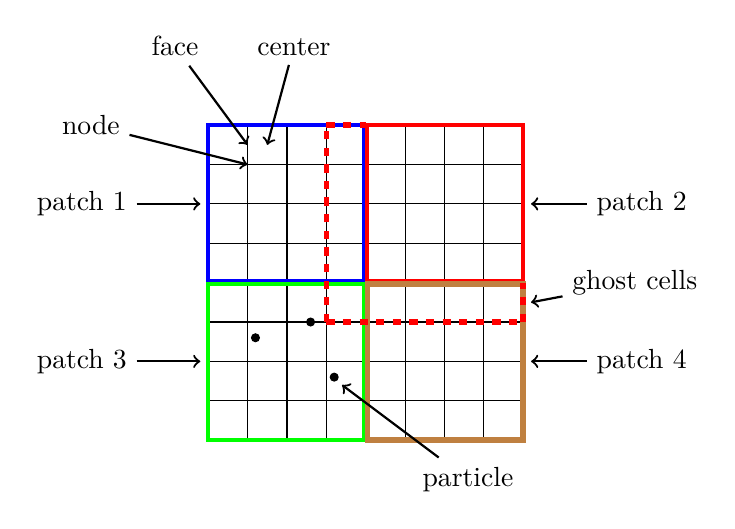
\begin{tikzpicture}
\node [anchor=east] (node) at (0,5) {node};
\node [anchor=east] (face) at (1,6) {face};
\node [anchor=west] (center) at (1.5,6) {center};
\node [anchor=west] (patch1) at (-1.3,4) {patch 1};
\node [anchor=east] (patch2) at (7.2,4) {patch 2};
\node [anchor=west] (patch3) at (-1.3,2) {patch 3};
\node [anchor=east] (patch4) at (7.2,2) {patch 4};
\node [anchor=east] (particle) at (5,0.5) {particle};
\node [anchor=west] (ghost) at (5.5,3) {ghost cells};
\draw [step=1] (1,1) grid (5,5);
\draw [step=0.5] (1,1) grid (5,5);
\draw [line width=1.5,color=blue] (1,3.02) rectangle (2.98,5);
\draw [line width=1.5,color=red] (3.02,3.02) rectangle (5,5);
\draw [line width=1.5,color=green] (1,1) rectangle (2.98,2.98);
\draw [line width=2,color=brown] (3.02,1) rectangle (5,2.98);
\draw [line width=2,color=red,dashed] (2.5,2.5) -- (5,2.5);
\draw [line width=2,color=red,dashed] (2.5,2.5) -- (2.5,5);
\draw [line width=2,color=red,dashed] (2.5,5) -- (3,5);
\draw [line width=2,color=red,dashed] (5,2.5) -- (5,3);
\draw [->,thick] (node) -- (1.5,4.5);
\draw [->,thick] (face) -- (1.5,4.75);
\draw [->,thick] (center) -- (1.75,4.75);
\draw [->,thick] (patch1) -- (0.9,4);
\draw [->,thick] (patch2) -- (5.1,4);
\draw [->,thick] (patch3) -- (0.9,2);
\draw [->,thick] (patch4) -- (5.1,2);
\draw [->,thick] (particle) -- (2.7,1.7);
\draw [->,thick] (ghost) -- (5.1,2.75);
\draw [fill] (2.3,2.5) circle [radius=0.05];
\draw [fill] (2.6,1.8) circle [radius=0.05];
\draw [fill] (1.6,2.3) circle [radius=0.05];
%\draw [black,decorate,decoration={brace,amplitude=5pt},
%   xshift=5pt,yshift=0pt] (5,5)  -- (5,3)
%   node [black,midway,below=-8pt,xshift=20pt] {AMR};
\end{tikzpicture}
\caption{A two dimensional view of the grid with its various components labeled.}
\label{fig:grid}
\end{figure}

One of the biggest reasons we chose to use the Uintah framework was that it has a very advanced \emph{parallel task system}. As already mentioned 
previously, in Uintah parallelization goes over patches. Every \emph{process} has \emph{N} patches which they are in charge of, and those patches 
are distributed according to load balancing settings. In our case, we chose to use a load balancing option that takes the number of particles into account. 

The parallel task system takes care of most data communication and working with data dependencies. For each \emph{function}, we must define a task which 
takes in the function, the function's \emph{dependencies} and the function's \emph{output}.

For instance, as we can see in the Equation 
\ref{eq:discretized_poisson}, for one poisson iteration, we need the \emph{last iteration's} $\phi=\phi_{previous}$ value as well as the distribution of 
particle density $\rho$, and one poisson iteration calculates the next $\phi=\phi_{next}$ value. Additionally, because according to Equation \ref{eq:discretized_poisson} 
we need neighbor values of every $\phi$ in our iterations, we need to tell the task that it needs to fetch 1 layer of \emph{ghost cells}. The concept of 
\emph{ghost cells} was demonstrated in Figure \ref{fig:grid}.

In pseudocode, this would be:
\begin{algorithm}[H]
 \begin{algorithmic}
  \State $Task \gets $new task($poissonIterationStep$)
  \State $Task \gets$ $\phi_{previous}$ with $1$ layer of \emph{ghost cells}
  \State $Task \gets$ $\rho_{current}$
  \State $Task$ \emph{computes} $\phi_{next}$
  \State $Scheduler \gets Task$
 \end{algorithmic}
 \caption{Demonstrating Uintah taskgraph system}
 \label{alg:uintah_task}
\end{algorithm}

In addition to tasks and different patch hierarchies, we may also explain the way Uintah parallelizes things, and why it is currently regarded as perhaps 
the most scalable grid library. Normally in most grid libraries, things advance in a \emph{semi-serial} way due to normal MPI programming. Whenever 
a function is done calculating, there is some communication between MPI processes (e.g. process \#1 needs to tell \#2 some result of a calculation). Until the 
communication is done, the process is often left hanging. This phenomena is often referred to as \emph{load imbalance}.

In the case of Uintah, the problem of load imbalance is overcome by introducing \emph{task dependencies}, which we already went through shortly in this section. 
Task dependencies refer to tasks having certain dependencies before they can be executed. For instance, say process \#1 can move to interpolating particle 
values to a grid or to calculating poisson iterations and poisson iteration still requires a variable which has not been calculated. In this case, the 
process \#1 would simply move on to interpolating particle values, instead of hanging around doing nothing, as would be the case in most normal parallel 
simulations.

For demonstration, we present a task graph taken from Uintah website in Figure \ref{fig:uintah_taskgraph}.

\begin{figure}[H]
 \centering
 \includegraphics[width=\textwidth]{Uintah/taskgraph.png}
 \caption{Task graph example from Uintah's website}
 \label{fig:uintah_taskgraph}
\end{figure}

In Uintah, there are essentially \emph{2} different ways to parallelize the simulation. Either one distributes the workload among \emph{processes}, or 
one distributes the workload among both \emph{processes} and \emph{threads}. We did not use the thread-based parallelization because unfortunately neither of 
our MPICH versions had support for the required level 3 parallelization, and tackling that problem simply requires too much of our valuable time. In fact, 
even FMI's supercomputer \emph{Voima} did not have support for level 3 paralllelization. We were still intrigued by the concept of making a \emph{hybrid-parallelization}, 
especially since our simulation should have it working out of the box, so we read more about it.

The way hybrid-parallelization in Uintah works is that every process is assigned $N$ threads, from which $1$ is used for MPI communication, and $N-1$ are 
used for execution of tasks. This should guarantee fast execution on supercomputers, as long as $N \approx 15-30$. Using hybrid-parallelization would 
reduce MPI communication, as threads within a process would have shared memory, and would not require for instance communication of ghost cells through 
MPI.

In addition to having a nice task-graph system, Uintah has put some effort into having general-use interfaces for implementing things. Patches can be sorted 
with \emph{Hilbert spatial filling curves}\footnote{Hilbert spatial filling curves are used to optimize memory cache. In the case of our simulation, cells 
are sorted in the way that neighbors of each cell are closer in memory, reducing cache misses in fetching neighbor cell data. For more information on 
space filling curves, see \url{http://www.diss.fu-berlin.de/diss/servlets/MCRFileNodeServlet/FUDISS_derivate_000000003494/2_kap2.pdf?hosts=}}, Uintah has tools for interpolating particles to nodes and nodes to particles and it has tools for calculating 
interpolated derivatives. Additionally, Uintah has support for implementing \emph{adaptive mesh refinement}\footnote{See Section \ref{sec:conclusions}}. 
Despite the fact that these tools have a steep learning curve, they will become invaluable when implementing parallel and optimized algorithms for 
mesh-based methods.

Finally, we will discuss some of the \emph{bugs and limitations} in Uintah. For one, interpolating particle and cell variables back and forth are viable only 
for node-based variables out-of-the-box. This is not unusual, as the visualization software \emph{VisIt} and most other mesh visualization softwares have 
a similar take on this. Making sparse data is also not possible in Uintah, meaning that solving e.g. \emph{Vlasov} equation on a sparse grid is not 
possible, and neither is solving many-dimensional partial differential equations with methods such as adaptive \emph{radial basis method}\footnote{Solving 
partial differential equations by assuming a basis of radial functions and often neglecting the functions which contribute less}. Additionally, there 
was one great limitation we encountered; the particle interpolation does not work when the particle variable has values around $1.0e40$. It gives spiked 
results for the interpolated variable, and it took us a day to find out this was why our simulation was producing incorrect results.

For some additional information, please refer to the Uintah presentation we 
made which can be found in:

\begin{verbatim}
./doc/Uintah/uintah_presentation.pdf
\end{verbatim}


\subsection{The program}

Now that we know the basics on Uintah, we can move on to looking at our program. Our main algorithm is described in the Algorithm \ref{alg:main}, 
and here we attempt to break this down into smaller details. All of this can 
be found also in our project files \emph{ParticleTest1.cc} and 
\emph{ParticleTest1.h}.

\emph{set Dirichlet or periodic boundary conditions}. Setting either dirichlet or periodic boundary conditions is fairly straightforward. 
In fact, this is something that we found Uintah can do for us. We need to 
simply input our boundary conditions in a run file and take it into account 
in our poisson solver. In our poisson solver, we simply skip iterating the 
cells that are on our grid border.

\emph{set initial $\mathbf{x}_p$, $\mathbf{v}_p$ and $m_p$ for all particles $p$}. 
For this purpose, Uintah specifies a function for initializing our data. We 
set particle position $\mathbf{x}_p=rand(grid)$, velocity $\mathbf{v}_p=0$ and mass $m_p = 1.0e4$. 

\emph{interpolate initial $\rho$ from particle mass $m_p$}. For this, we use 
linear interpolation method. Our $\rho$ is specified at each cell corner 
(\emph{node}\footnote{See section \ref{ssec:Uintah}}) and we interpolate 
the particle mass variable to nearest $8$ nodes. Since $\rho$ is density, we 
also divide the interpolated mass variable by one cell volume $\Delta x \Delta y \Delta z$. 
The reason we chose to interpolate only to $8$ nearest nodes (e.g. 
use linear interpolation) is because it can be shown with some effort that this is produces a sufficient accuracy 
for the Poisson equation. By sufficient, 
we of course mean that it does not introduce a global error of higher order 
than what is already in our simulation due to discretizing poisson equation.
For this purpose, we 
found that Uintah has a class called \emph{ParticleInterpolator} that 
produces interpolation. This required us to change our $\rho$ variable to 
node-centered form from cell-centered form, however. This method is widely 
used for communication between grids and particles, and commonly methods 
using this are referred to as a \emph{cloud-in-cell} or \emph{particle-in-cell} 
methods.

\emph{set initial guess for $\phi$}. We set this to zero everywhere.

\emph{solve $\phi$ at the nodes}. For this, we created an iterative solver 
that goes through each patch\footnote{See Section \ref{ssec:Uintah}} and 
iterates through each \emph{node} in that patch. Basically, we solve 
the Equation \ref{eq:discretized_poisson}. We require that each patch 
fetches $1$ layer of \emph{ghost nodes}\footnote{See Section \ref{ssec:Uintah}} 
to deal with patch boundaries, as our algorithm needed the neighboring nodes\footnote{neighboring node = node which is one node to the left,right,down,up,forward or backward} 
for each node. Additionally, we skip the cells at the patch \emph{boundaries} due 
to boundary conditions. Our algorithm for solving the poisson 
equation is demonstrated in Algorithm \ref{alg:Jacobi}. For every iteration, we also 
created a task to utilize the full functionality of \emph{Uintah}. For task dependencies in the Poisson solver, please refer to Algorithm 
\ref{alg:uintah_task}.

\emph{calculate $\mathbf{F}=-\nabla \phi$ for each particle $p$}. For this, 
we use linear interpolation. For every particle $p$, we pick the $8$ nearest 
nodes and interpolate to values $x_i+dx_i$ and $x_i-dx_i$ for every $i$. 
This means that our gradient calculation is also based on linear interpolation. 
This introduces some error, but again it has been shown to be sufficient 
for solving poisson equation.

\emph{propagating every particle p}. This is already documented in 
Algorithm \ref{alg:main}, so we do not elaborate it further here.

\emph{interpolate new $\rho$ from particle mass $m_p$}. See the step 
\emph{interpolate initial $\rho$ from particle mass $m_p$}.

\emph{$t \gets t + \Delta t$}. This is done in the Uintah framework 
and is determined by the variable $Delt$ in the runtime \emph{XML} file. 
We use constant timestepping, so this step needs nothing complicated.


\section{RESULTS}

\subsection{Movies}

We present movies separately from this report. They are one of the main results of this whole study, however, as they demonstrate 
perhaps the best way how our simulation works dynamically. These movies can be found in the \emph{movies} folder.

\subsection{Dark matter halo}

Here we present the dark matter halo in our simulation at an Equilibrium. For a better view of the dynamics of the whole process, please see our 
movies of different simulation runs.

\begin{figure}[H]
\centering
\includegraphics[width=.8\textwidth]{dm_halo.png}
\caption{Our simulation run with periodic boundary conditions and a formed halo. The simulation time step is chosen from a point when the halo shape 
is at an equilibrium.}
\label{fig:dm_halo}
\end{figure}

\subsection{Energy conservation and virial theorem}

We want to make sure that energy is conserved in our simulation and we compare it with the virial theorem. Energy conservation is somewhat difficult to do because 
of the weird units we were forced to use which were Section \ref{sec:methods} (namely $G=1$).

For simplicity, we calculate a \emph{scaling factor} $C$ for comparing units of $\phi$ and $|\mathbf{v}|^2$ by using the virial theorem:

$<v^2>_\tau = C <\phi>_\tau$

In other words, $C * \phi$ is simply $\phi$ in same magnitudes as $v^2$. As for why we need to do this is because Uintah simply does not have support for 
interpolating large values back and forth, as mentioned in Section \ref{ssec:Uintah}.

We then compare energy conservation by comparing different timesteps' total energy:

$[0.5v^2+C\phi]_{t=t_1} - [0.5v^2+C\phi]_{t=t_2} = Error$

In this case, we only look at $10$ timesteps.

The results are presented here and under \newline \emph{./doc/results/energyConservation/virialTheoryAndEnergyConservationResults.dat}:


\begin{verbatim}
Scaling factor, calculated from virial theorem: -2.00313776377e-05
Energy conservation at timestep 140; potential: 2171895072.08, v_squared: 2189590262.88
Total Energy: 4361485334.96
Energy conservation at timestep 141; potential: 2171448825.2, v_squared: 2177912632.04
Total Energy: 4349361457.24
Energy conservation at timestep 142; potential: 2171267304.94, v_squared: 2148816440.27
Total Energy: 4320083745.2
Energy conservation at timestep 143; potential: 2170731390.9, v_squared: 2188656985.4
Total Energy: 4359388376.3
Energy conservation at timestep 144; potential: 2169414726.35, v_squared: 2172310920.46
Total Energy: 4341725646.81
Energy conservation at timestep 145; potential: 2167363889.69, v_squared: 2150885442.1
Total Energy: 4318249331.79
Energy conservation at timestep 146; potential: 2165176115.51, v_squared: 2152619861.33
Total Energy: 4317795976.84
Energy conservation at timestep 147; potential: 2163085388.64, v_squared: 2172501600.59
Total Energy: 4335586989.23
Energy conservation at timestep 148; potential: 2161168195.91, v_squared: 2178308681.32
Total Energy: 4339476877.23
Energy conservation at timestep 149; potential: 2159870013.0, v_squared: 2139818095.83
Total Energy: 4299688108.84
\end{verbatim}

It looks as though our energy is not conserved perfectly, but it is in the right orders of magnitude. The largest change (between first and last timestep) for 
example is merely $E_{diff}=61797226$, whose relative value is $61797226/4299688108 \approx 0.014$. We assume this depends on both the choice of $dt$ and 
\emph{resolution} in our algorithm. This will be discussed in the Section \ref{sec:conclusions}.

\subsection{NFW profile}

As mentioned in Section \ref{sec:verification}, the dark matter halo density profiles should follow the \emph{NFW} profile given in Equation \ref{eq:nfw}. 
This is when a dark matter halo has reached an equilibrium, so at a timestep quite far away in the simulation. We made multiple runs, of which we will use 
the run which used $50^3$ cells and $150000$ particles and periodic boundary conditions. We take a line-out plot of the dark matter density $\rho$ and 
compare it with the \emph{NFW} profile.

\begin{figure}[H]
\centering
\includegraphics[width=.8\textwidth]{NFW_profile.pdf}
\caption{The shape of the radial distribution of mass density suggested by NFW profile (Equation \ref{eq:nfw}), choosing $\rho_0=1$ and $R_s=1$.}
\label{fig:nfw}
\end{figure}

\begin{figure}[H]
\centering
\includegraphics[width=.8\textwidth]{NFW-profile.png}
\caption{Line-out from our simulation. The line-out starts from the center of the dark matter halo}
\label{fig:simulationnfw}
\end{figure}

From comparing at Figures \ref{fig:nfw} and \ref{fig:simulationnfw} we simply conclude that the NFW profile could be fitted into the profile of the dark matter 
halo. Our peak is not as strong as we have a discretized grid which prevents our values from hitting $\infty$. Obviously, the Figure \ref{fig:nfw} is only 
a plot of the \emph{NFW} profile with coefficients we picked by ourselves. We show it mainly to give the reader a general view of the shape of the 
\emph{NFW} profile.

Our initial 
plan was to actually fit the Equation \ref{eq:nfw} into our simulation, but unfortunately \emph{VisIt} visualization tool could not allow us to 
extract variables from a lineout plot so we could do it in Python. Hence, we instead compared to make sure the \emph{NFW} profile's shape correlated 
with our lineout plot

\subsection{Scalability}

With the boasted great scalability in Uintah, we decided to run our code on the supercomputer \emph{Voima}. For parallelization, we used an MPI-based 
approach, so we use processes for parallelizing the threads and use $1$ thread per process. This is due to lack of support for level $3$ parallelization in 
Voima's \emph{MPICH} library. According to various sources, this could be fixed either by compiling MPICH again from source with different configuration 
settings or possibly by tampering with some flags. Anyway, we made scalability tests with 10,20,30,40,50,60 and 70 nodes by running a simple test 
case with $5$ million particles, $300^3$ cells and $5^3$ patches. The log file of the runs is presented in the \emph{Uintah\_run\_information} 
folder of the root folder. 

For results, we present Figures \ref{fig:scalability1}, \ref{fig:scalability2}.

\begin{figure}[H]
\centering
\includegraphics[width=\textwidth]{Uintah/scalability.png}
\caption{Scalability test for our simulation. We ran the simulation with $5$ million particle and $300^3$ cells.}
\label{fig:scalability1}
\end{figure}

\begin{figure}[H]
\centering
\includegraphics[width=\textwidth]{Uintah/scalability2.png}
\caption{Scalability test for our simulation. We ran the simulation with $5$ million particle and $300^3$ cells. The speed-up is counted relative to 
10 cores}
\label{fig:scalability2}
\end{figure}

Most notably, we see a speed-up of over $8$ in Figure \ref{fig:scalability2}. This can only be explained by some memory optimizations in different 
processes running on different cores. For example, it is known that with large datasets and with large memory usage, \emph{cache misses} become more frequent as 
large jumps in memory become more frequent.

We would have also tested for \emph{hybrid parallelization} by employing both processes and threads, but unfortunately that would have required 
tampering with the MPICH library, which would have cost quite a bit of time.

% visit figure:
% initial vs final condition
% mp4 movie...

\section{CONCLUSIONS} \label{sec:conclusions}
This project had two main purposes. Firstly we simulated a dark matter halo by solving the Poisson's equation of gravity coupled with dark matter particles in the framework provided by Uintah. Secondly, and perhaps more importantly, we learned to use some of the powerful tools provided by Uintah that provide parallelized and optimized grid framework for solving a multitude of problems in computational physics.

The simulation results are physically sound as they comply with energy conservation and virial theorem and reproduce a mass density distribution similar to other simulations.

One important Uintah tool that we did not utilize due to time constratints is adaptive mesh refinement (AMR). This essentially means that based on some predefined condition(s) specified in the simulation, the resolution would be increased in some parts of the grid. This would let us emphasize interesting regions in the simulation and de-emphasize less interesting regions. This also means that the simulations becomes computationally more efficient. AMR is something we wish to explore more in the future.

NFW profile could be fitted to the data from our simulation to find out the parameters $(\rho_0,R_s)$. These parameters could then be compared with other studies. We also want to make the simulation with proper units and realistic scale, this would probably mean solving some problems with the Uintah interpolator. Also the the effect of resolution on the accuracy of the results could be studied more extensively, both analytically and numerically. 

        

\section{RUNNING, COMPILING AND DOING THINGS WITH UINTAH}

In the requirements for the course, it was encouraged to add the software used into the project folder. We will not do this, as Uintah is a large code 
that has some $\approx 700k$ lines of code. Additionally, to analyze the files one needs to compile \emph{VisIt} from source with the --uintah option 
in order to read the \emph{.uda} file format. 


In other words, installing Uintah can be done by first downloading it, taking a 2-10 hours to install all dependencies needed to compile it, then compile it 
(the compilation will take another hour) and then you need to install VisIt from source. By the time you have Uintah installed, you should have most 
of the dependencies worked out, though, so it's a bit easier. Downloading all the stuff that \emph{VisIt} uses will take approx an hour as well, though, and 
compiling VisIt takes about an hour.

For us, this took about 2 days, but then again we had some major dependency issues.

\subsection{Installing instructions}

Step 1 Download Uintah

Step 2 Compile Uintah in a build folder

Step 3 Download VisIt

Step 4 Install VisIt from source using the --uintah option

Step 5 You're done
        
% what should we do next?

\renewcommand{\refname}{REFERENCES}
\begin{thebibliography}{}
\bibitem[Kuhlen et al., 2012]{Kuhlen2012}
Kuhlen, M. et al., (2012),
\newblock{Numerical Simulations of the Dark Universe: State of the Art and the Next Decade},
\newblock{arXiv:1209.5745 [astro-ph, physics:hep-ph]}
\bibitem[Roos, 2012]{Roos2010}
Roos, M., (2010),
\newblock{Dark Matter: The evidence from astronomy, astrophysics and cosmology},
\newblock{arXiv:1001.0316 [astro-ph]}
\bibitem[Hockeny and Eastwood, 1985]{Hockney1985}
Hockney, R.W. and Eastwood, J.W., (1985),
\newblock{Computer Simulation Using Particles},
\newblock{CRC Press}
\bibitem[Navarro et al., 1995]{Navarro1995}
Navarro, F.N. et al., (1995),
\newblock{The Structure of Cold Dark Matter Halos},
\newblock{arXiv:astro-ph/9508025}
\end{thebibliography}
\end{document}
